\documentclass[a4paper,12pt,fleqn]{article}

\usepackage{amsmath}
\usepackage[margin=1in]{geometry}
\usepackage{xcolor}
\usepackage{tikz}
\usepackage{subcaption}
\usepackage[hypertexnames=false,bookmarksnumbered=true,final]{hyperref}
\usepackage[capitalize,sort]{cleveref}
\usetikzlibrary{decorations.pathreplacing,arrows.meta,calc,3d,perspective}

\def\colorschemesepia{sepia}
\def\colorschemedark{dark}
\def\colorschemelight{light}

\ifx\colorscheme\undefined
\let\colorscheme\colorschemelight
\fi

\ifx\colorscheme\colorschemelight
\colorlet{textColor}{black}
\colorlet{bgColor}{white}
\fi

\ifx\colorscheme\colorschemesepia
\definecolor{textColor}{HTML}{433423}
\definecolor{bgColor}{HTML}{fbf0da}
\fi

\ifx\colorscheme\colorschemedark
\definecolor{textColor}{HTML}{bdc1c6}
\definecolor{bgColor}{HTML}{202124}
\colorlet{textHeavy}{white}
\definecolor{textRed}{HTML}{ff968c}  % hsb(5 deg, 45%, 100%)
\definecolor{textGreen}{HTML}{70cc70}  % hsb(120 deg, 45%, 80%)
\definecolor{textBlue}{HTML}{8cbcff}  % hsb(215 deg, 45%, 100%)
\definecolor{textCyan}{HTML}{70cccc}  % hsb(180 deg, 45%, 80%)
\definecolor{textMagenta}{HTML}{d982d9}  % hsb(300 deg, 40%, 85%)
\definecolor{textYellow}{HTML}{bfbf69}  % hsb(60 deg, 45%, 75%)
\else
\colorlet{textHeavy}{black}
\colorlet{textRed}{red!50!black}
\colorlet{textGreen}{green!50!black}
\colorlet{textBlue}{blue!50!black}
\colorlet{textCyan}{cyan!80!black}
\colorlet{textMagenta}{magenta!80!black}
\colorlet{textYellow}{yellow!60!black}
\definecolor{textPurple}{HTML}{681da8}
\fi

\colorlet{dimColor}{textColor!50!bgColor}

\ifx\colorscheme\colorschemelight\else
\pagecolor{bgColor}
\color{textColor}
\fi

%\hypersetup{colorlinks,linkcolor=textRed,citecolor=textRed,urlcolor=textBlue}

\hypersetup{colorlinks,linkcolor=textRed,citecolor=textRed,urlcolor=textBlue}

\DeclareMathOperator{\opt}{opt}
\let\eps\varepsilon

\title{Bin Packing}
\author{\empty}
\date{\empty}

\begin{document}

\maketitle
\setlength{\parskip}{0.5em}

\section{Introduction}

In the classical bin packing problem, we are given a set $I$ of items.
Each item $i \in I$ has a size $s(i) \in (0, 1]$ associated with it.
Our goal is to partition $I$ into the minimum number of bins,
such that the sum of sizes of items in each bin is at most 1.
See \cref{fig:1bp} for an example.
The classical bin packing problem and its generalizations
have diverse applications in computer science and operations research,
like packing goods into trucks, allocating jobs to servers,
allocating memory in computers~\cite{handbook-of-combinopt-bp},
or assigning advertisements to station breaks in television programming.

\begin{figure}[!ht]
\centering
\begin{subfigure}{0.9\textwidth}
    \centering
    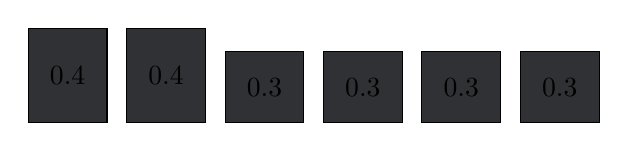
\begin{tikzpicture}[item/.style={fill={textColor!10!bgColor},draw}]
\path[item]
    (0,0) rectangle +(1,1.2) node[pos=0.5] {0.4}
    ++(1.25,0) rectangle +(1,1.2) node[pos=0.5] {0.4}
    ++(1.25,0) rectangle +(1,0.9) node[pos=0.5] {0.3}
    ++(1.25,0) rectangle +(1,0.9) node[pos=0.5] {0.3}
    ++(1.25,0) rectangle +(1,0.9) node[pos=0.5] {0.3}
    ++(1.25,0) rectangle +(1,0.9) node[pos=0.5] {0.3};
\end{tikzpicture}

    \caption{A set of six items: two items have size 0.4 and four items have size 0.3.}%
\label{fig:1bp:a}
\end{subfigure}
\par\bigskip\bigskip
\begin{subfigure}{0.45\textwidth}
    \centering
    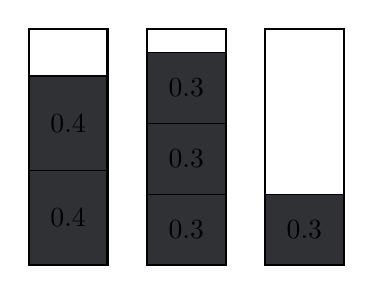
\begin{tikzpicture}[
item/.style={fill={textColor!10!bgColor},draw},
bin/.style={draw,thick},
]
\path[item]
    (0.0,0.0) rectangle +(1,1.2) node[pos=0.5] {0.4}
    (0.0,1.2) rectangle +(1,1.2) node[pos=0.5] {0.4}
    (1.5,0.0) rectangle +(1,0.9) node[pos=0.5] {0.3}
    (1.5,0.9) rectangle +(1,0.9) node[pos=0.5] {0.3}
    (1.5,1.8) rectangle +(1,0.9) node[pos=0.5] {0.3}
    (3.0,0.0) rectangle +(1,0.9) node[pos=0.5] {0.3};
\path[bin]
    (0,0) rectangle +(1,3)
    ++(1.5,0) rectangle +(1,3)
    ++(1.5,0) rectangle +(1,3);
\end{tikzpicture}

    \caption{A packing of the items into 3 bins.}
\end{subfigure}
\begin{subfigure}{0.45\textwidth}
    \centering
    \input{img/1bp-c.tikz}
    \caption{A packing of the items into 2 bins.}
\end{subfigure}
\caption[An example of classical bin packing.]{An example of classical bin packing.
We want to minimize the number of bins, so the packing into 2 bins
is better than the packing into 3 bins.}
\label{fig:1bp}
\end{figure}

First-Fit Decreasing (FFD) is a popular algorithm for classical bin packing.
Johnson~\cite{johnson-thesis} showed that the number of bins used by
FFD is at most $(11/9)\opt(I) + 4$,
where $\opt(I)$ is the minimum number of bins needed to pack $I$.
Lueker and Vega~\cite{bp-aptas} gave an algorithm that accepts a parameter $\eps > 0$
and packs the items into $(1+\eps)\opt(I) + O(1/\eps^2)$ bins in $O(n\log n + 1/\eps^2)$ time.

In the 2-dimensional geometric bin packing problem (abbreviated as 2D GBP),
we are given a set $I$ of $n$ rectangular items and an infinite supply
of identical rectangular bins.
Our task is to pack the rectangles into the minimum number of bins such that
in each bin, the items don't overlap.
See \cref{fig:2gbp} for an example.

\begin{figure}[htb]
\centering
% define colors
\def\rangeHsb{15}
\foreach \n in {0,...,14}
{\xglobal\definecolor{hue\n}{rgb:Hsb}{\n,1,1}%
\xglobal\colorlet{myColor\n}{hue\n!20!bgColor}}
\colorlet{lineColor}{textColor!75!bgColor}
%
\newlength{\myunit}
\setlength{\myunit}{0.325cm}
\begin{tikzpicture}[scale=0.7,
bin/.style={draw=lineColor,thick},
item/.style={draw=lineColor},
myarrow/.style={draw=lineColor,->,>={Stealth},thick},
]
\begin{scope}[yshift=2.1cm]
\path[item,fill=myColor0] (1\myunit, 19\myunit) rectangle +(7\myunit, 7\myunit);
\path[item,fill=myColor1] (7\myunit, 0\myunit) rectangle +(9\myunit, 6\myunit);
\path[item,fill=myColor2] (0\myunit, 1\myunit) rectangle +(6\myunit, 9\myunit);
\path[item,fill=myColor3] (7\myunit, 7\myunit) rectangle +(8\myunit, 3\myunit);
\path[item,fill=myColor4] (9\myunit, 19\myunit) rectangle +(4\myunit, 7\myunit);
\path[item,fill=myColor5] (13\myunit, 11\myunit) rectangle +(3\myunit, 7\myunit);
\path[item,fill=myColor6] (0\myunit, 11\myunit) rectangle +(12\myunit, 2\myunit);
\path[item,fill=myColor7] (2\myunit, 16\myunit) rectangle +(9\myunit, 2\myunit);
\path[item,fill=myColor8] (17\myunit, 1\myunit) rectangle +(2\myunit, 9\myunit);
\path[item,fill=myColor9] (17\myunit, 11\myunit) rectangle +(2\myunit, 7\myunit);
\path[item,fill=myColor10] (14\myunit, 23\myunit) rectangle +(4\myunit, 4\myunit);
\path[item,fill=myColor11] (14\myunit, 19\myunit) rectangle +(5\myunit, 3\myunit);
\path[item,fill=myColor12] (0\myunit, 14\myunit) rectangle +(12\myunit, 1\myunit);
\end{scope}
\draw[myarrow] (19\myunit+0.5cm,6.45cm) -- (10cm-0.5cm,6.45cm);
\begin{scope}[xshift=10cm]
\begin{scope}[yshift=9cm]
\path[item,fill=myColor2] (0\myunit, 3\myunit) rectangle +(6\myunit, 9\myunit);
\path[item,fill=myColor5] (8\myunit, 3\myunit) rectangle +(3\myunit, 7\myunit);
\path[item,fill=myColor6] (0\myunit, 0\myunit) rectangle +(12\myunit, 2\myunit);
\path[item,fill=myColor8] (6\myunit, 3\myunit) rectangle +(2\myunit, 9\myunit);
\path[item,fill=myColor12] (0\myunit, 2\myunit) rectangle +(12\myunit, 1\myunit);
\path[bin] (0\myunit, 0\myunit) rectangle (12\myunit, 12\myunit);
\end{scope}
\begin{scope}[yshift=4.5cm]
\path[item,fill=myColor1] (0\myunit, 0\myunit) rectangle +(9\myunit, 6\myunit);
\path[item,fill=myColor3] (0\myunit, 8\myunit) rectangle +(8\myunit, 3\myunit);
\path[item,fill=myColor7] (0\myunit, 6\myunit) rectangle +(9\myunit, 2\myunit);
\path[item,fill=myColor9] (9\myunit, 0\myunit) rectangle +(2\myunit, 7\myunit);
\path[bin] (0\myunit, 0\myunit) rectangle (12\myunit, 12\myunit);
\end{scope}
\begin{scope}
\path[item,fill=myColor0] (0\myunit, 0\myunit) rectangle +(7\myunit, 7\myunit);
\path[item,fill=myColor4] (7\myunit, 0\myunit) rectangle +(4\myunit, 7\myunit);
\path[item,fill=myColor10] (0\myunit, 7\myunit) rectangle +(4\myunit, 4\myunit);
\path[item,fill=myColor11] (4\myunit, 7\myunit) rectangle +(5\myunit, 3\myunit);
\path[bin] (0\myunit, 0\myunit) rectangle (12\myunit, 12\myunit);
\end{scope}
\end{scope}
\end{tikzpicture}

\caption{Packing 13 rectangles into 3 bins (without rotation).}
\label{fig:2gbp}
\end{figure}

There are two commonly-studied versions of 2D GBP.
In the non-rotational version, rotating the items is forbidden.
In the rotational version, the items can be rotated by $90^{\circ}$.
In both versions, the items and bins are oriented parallel to the coordinate axes.

2D GBP finds applications in the wood-cutting, metal-cutting, paper and cloth industries,
where rectangular pieces need to be cut out of standard-sized sheets,
and item rotations are usually allowed.
Non-rotational 2D GBP can be used for placing advertisements on web pages and newspapers.

For 2D GBP (both rotational and non-rotational versions),
Bansal and Khan's algorithm~\cite{bansal2014binpacking}
packs the items into $(\alpha+\eps)\opt(I)+O(1)$ bins, where
$\alpha = 1 + \ln(1.5) \approx 1.4055$.

\bibliographystyle{plainurl}
\bibliography{bibdb}

\end{document}
